\documentclass[a4paper,english]{lipics-v2019}
\usepackage{wrapfig,microtype,amssymb,amsmath,stmaryrd,mathpartir,array,graphicx,tabularx,xspace}
\usepackage[table]{xcolor}
\newcommand{\xt}[1]{\texttt{#1}}
%\newcommand{\tupleo}[1]{\xt{Tuple1\{}#1\xt{\}}}
\newcommand{\tuplet}[2]{\xt{Tuple\{}#1,#2\xt{\}}}
\newcommand{\union}[2]{\xt{Union\{}#1,#2\xt{\}}}
\newcommand{\denotes}[1]{\llbracket #1 \rrbracket}

\renewcommand{\L}{{\tt L}\xspace}
\newcommand{\Ls}{{\tt L}s\xspace}
\newcommand{\R}{{\tt R}\xspace}
\newcommand{\Rs}{{\tt R}s\xspace}
\newcommand{\uL}{{\underline{\tt L}}\xspace}
\renewcommand{\c}[1]{\ensuremath{\text{\lstinline{#1}}}\xspace}

%FZ
\newcommand{\sub}{<:}
\newcommand{\tuple}[1]{\xt{Tuple\{}#1\xt{\}}}
\newcommand{\arrayt}[1]{\xt{Array\{}#1\xt{\}}}
\newcommand{\FZ}[1]{\textbf{FZ says: #1}}
%end FZ

\newcommand{\goodcell}{\cellcolor{green!25}}
\newcommand{\badcell}{\cellcolor{red!25}}
\bibliographystyle{plainurl}% the recommnded bibstyle
\title{Julia's efficient algorithm for subtyping unions and covariant tuples}
\titlerunning{Subtyping union types and covariant tuples}

\author{Benjamin Chung}{Northeastern University}{}{}{}%mandato
\author{Francesco Zappa Nardelli}{INRIA}{}{}{} \author{Jan
  Vitek}{Northeastern University \& Czech Technical University in
 Prague}{}{}{}
\authorrunning{B. Chung, F. Zappa Nardelli, J. Vitek}
\Copyright{Benjamin Chung, Francesco Zappa Nardelli, Jan Vitek}%mandatory, plea
\ccsdesc[500]{Theory of computation~Type theory}
\keywords{Type systems, Subtyping, Union types}

\lstset{
 language=caml,
 columns=[c]fixed,
 basicstyle=\small\ttfamily,
 keywordstyle=\bfseries,
 upquote=true,
 commentstyle=,
 breaklines=true,
 showstringspaces=false}

%Editor-only macros:: begin (do not touch as author)%%%%%%%%%%%%%%%%%%%%%%%%%%%%%%%%%%
\EventEditors{John Q. Open and Joan R. Access}
\EventNoEds{2}
\EventLongTitle{42nd Conference on Very Important Topics (CVIT 2016)}
\EventShortTitle{ECOOP}
\EventAcronym{ECOOP}
\EventYear{2019}
\EventDate{December 24--27, 2016}
\EventLocation{Little Whinging, United Kingdom}
\EventLogo{}
\SeriesVolume{42}
\ArticleNo{23}
%%%%%%%%%%%%%%%%%%%%%%%%%%%%%%%%%%%%%%%%%%%%%%%%%%%%%%

\begin{document}

\maketitle
\begin{abstract}
  The Julia programming language supports multiple dispatch and provides a
  rich type annotation language to specify method applicability. When
  multiple methods are applicable for a given call, Julia relies on
  subtyping between method signatures to pick the method to invoke. Julia's
  subtyping algorithm is surprisingly complex, and deciding whether it is
  correct remains an open question. In this paper, we focus on a piece of
  the problem, the interaction between union types and covariant
  tuples. Previous work that addressed this particular combination of
  features did so by normalizing types to a disjunctive normal form
  ahead-of-time. Normalization is not practical due to space-explosion for
  complex type signatures and to interactions with other features of Julia's
  type system.  Our contribution is a description of the algorithm
  implemented in the Julia run-time system. This algorithm is immune to the
  space-explosion and expressiveness problems of standard algorithms.  We
  prove this algorithm correct and complete against a semantic-subtyping
  denotational model in Coq.
\end{abstract}

\section{Introduction}

Union types, originally introduced by Barbanera and
Dezani-Ciancaglini~\cite{barbanera1991intersection}, are increasingly being
used in mainstream languages. In some cases, as Julia~\cite{BezansonEKS17}
or TypeScript~\cite{typescript}, they are exposed at the source level. In
others, such as Hack~\cite{hack}, they are only used internally when
performing type inference. We describe a space-efficient technique for
computing subtyping between types in the presence of distributive unions.
Our motivation arises from the Julia programming language. In our previous
work on formalizing the Julia subtyping
algorithm~\cite{DBLP:NardelliBPCBV18}, we described the subtyping relation
but were unable to describe the subtyping algorithm or prove it
correct. Indeed, we found bugs and were left with unresolved issues.

Julia's subtyping algorithm is an important part of its semantics. Julia is
a dynamically typed language where methods are annotated with type
signatures to enable multiple dispatch. During program execution, Julia must
determine which method to invoke at each call site. It does so by finding
the most specific applicable method (according to subtyping) that applies
for a given invocation. The following snippet shows three declarations of
multiplication.

\begin{lstlisting}
 *(x::Number, r::Range)  = range(x*first(r),...)
 *(x::Number, y::Number) = *(promote(x,y)...)
 *(x::T, y::T) where T <: Union{Signed,Unsigned} =  mul_int(x,y)
\end{lstlisting}

\noindent The first two methods implement, respectively, the case where a
range is multiplied by a number and generic numeric multiplication. The
third method invokes native multiplication when both arguments are either
signed or unsinged integers (but not a mix of the two).

Julia offers programmers a rich type language, including nominal single
subtyping, union types, existential types, covariant tuples, invariant
parametric datatypes, and singleton types. These features are widely used in
libraries, but pose challenges for subtyping. The design of subtyping was
inspired by semantic subtyping~\cite{Frisch02,BezansonEKS17}, but Julia
departs from that intuitive understanding of  the meaning of types.

This paper documents the first steps towards proving the correctness of
Julia's subtyping algorithm. We focus on the interaction of two features:
union types and covariant tuples. Tuples are used to represent function
signatures (Julia does not record return types). They are covariant as a
function with more specific arguments is preferred to a more generic one.
Union types are used as shorthand to avoid having to write multiple
functions with the same body.  Rules for subtyping union types and covariant
tuples have been known for a long time. Based on Vouillon~\cite{Vouillon04},
the following is a typical deductive system:

\vspace{-3mm}{\small\begin{mathpar}
\inferrule[allexist]{
   t' \sub t \\ t'' \sub t}{\union{t'}{t''} \sub t}

\inferrule[existL]{t \sub t'}{t \sub \union{t'}{t''}}

\inferrule[existR]{t \sub t''}{t \sub \union{t'}{t''}}

\inferrule[tuple]{t_1 \sub t'_1 \\ t_2 \sub t'_2}{\tuple{t_1, t_2} \sub \tuple{t'_1, t'_2}}
\end{mathpar}}
\vspace{-3mm}

\noindent While this rule system makes sense, it does not match the
intuition for subtyping. If we think of types as sets of
values~\cite{Pierce1991}, we would expect that a union type would be
analogous to set theoretic union. Similarly, we would then expect that two
types would be subtypes if their sets of values were subsets.  Therefore,
when a union type appears on the left-hand side of a judgment, \emph{all}
its components must be subtypes of the right-hand side; when a union type
appears on the right-hand side of a judgment, there must \emph{exist} a
component that is a supertype of the left-hand side. The above
system of rules violates these ideas. Consider the following judgment:

%
\vspace{-3mm}{\small\[
\tuple{\union{t'}{t''}, t} \ \ \sub\ \ \union{\tuple{t', t}}{\tuple{t'', t}} 
\]}
\vspace{-3mm}
%

\noindent Under a semantic subtyping, the judgment should hold. We write the
set of values denoted by the type $t$ as {\small $\llbracket t \rrbracket$}.
The left hand side denotes the values {\small $\{\tuple{v',v''} ~|~ v' \in
  \llbracket t' \rrbracket \cup \llbracket t'' \rrbracket \wedge v'' \in
  \llbracket t \rrbracket\}$}, while the right hand side denotes {\small
  $\llbracket \tuple{t', t} \rrbracket \cup \llbracket \tuple{t'', t}
  \rrbracket$}.  Obviously, the sets are the same. However, we cannot derive
this relation from the above rules. According to them, we must pick either
{\small $t'$} or {\small $t''$}, ending up with either {\small
  $\tuple{\union{t'}{t''}, t} \sub \tuple{t', t}$} or {\small
  $\tuple{\union{t'}{t''}, t} \sub \tuple{t'', t}$}. In either case, the
judgment does not hold.

Some early work~\cite{barbanera1991intersection,Pierce1991} uses
normalization to decide distributive subtyping between union types, while
Vouillon~\cite{Vouillon04} does not handle distributivity. Normalization
entails rewriting all types into their disjunctive normal form, as unions of
union-free types, \emph{before} building the derivation. This lifts all
choices to the top level, avoiding the structural entanglements that cause
trouble. The correctness of this rewriting step is justified by the
semantic-subtyping denotational model~\cite{Frisch08}, and the resulting
subtype algorithm can be proved both correct and complete. However, this
algorithm has two major drawbacks: it is not space efficient and it does not
interact well with other features of Julia..

The first drawback is that the normalization can lead to exponentially
bigger types. Real-world Julia code has types like the
following~\cite{DBLP:NardelliBPCBV18} whose normal form has 32,768
constituent base types, making it impractical to store or to compute with:


\begin{small}
\begin{verbatim}
 Tuple{Tuple{Union{Int64, Bool}, Union{String, Bool}, Union{String, Bool}, 
             Union{String, Bool}, Union{Int64, Bool}, Union{String, Bool}, 
             Union{String, Bool}, Union{String, Bool}, Union{String, Bool}, 
             Union{String, Bool}, Union{String, Bool}, Union{String, Bool}, 
             Union{String, Bool}, Union{String, Bool}, Union{String, Bool}}, Int64}
\end{verbatim}
\end{small}

The second drawback of normalisation is that it does not interact well with
other features of the type system. For instance, Julia supports invariant
constructors, which are incompatible with union normalization. For example,
the type $\arrayt{\xt{Int}}$ is an array of integers, this type is not be a
subtype of $\arrayt{\xt{Any}}$. This seemingly simple feature, in
conjunction with type variables, makes normalization ineffective.
Consider the type {\small \(\arrayt{\union{t'}{t''}}\)}. This type denotes the set
of arrays whose elements are either of type {\small $t'$} or {\small   $t''$}.
It would be incorrect to rewrite it as {\small
\(\union{\arrayt{t'}}{\arrayt{t''}}\)}, as this latter type denotes the set of
arrays whose elements are either all of type {\small $t'$} or all of type
{\small$t''$}. A weaker disjunctive normal form, only lifting union types
inside each invariant constructor, can circumvent this problem. However, doing
so only to reveals a deeper problem in thfe presence of both invariant
constructors and {existential types}. This is illustrated by the following judgment:

%
\vspace{-3mm}{\small\[
  \arrayt{\union{\tuple{t}}{\tuple{t'}}} \ \ <:\ \ \exists T\,.\, \arrayt{\tuple{T}}
\]}\vspace{-3mm}
%

\noindent 
This judgment holds if we set the existential {\small$T=\union{t}{t'}$}.
Since all types are in weak normal form, an algorithm based on the standard
system of judgment rules would strip off the array type constructors and
proceed.  However, since type constructors are invariant on their arguments,
it must first test that the relation holds in the original order (e.g. that
$\union{\tuple{t}}{\tuple{t}} <: \tuple{T}$) and in the reverse order (that
$\tuple{T} <: \union{\tuple{t}}{\tuple{t'}}$). It is in this combined check
that we run into problems.
%
The original order subtype check can be concluded without issue, producing
the constraint on $T$ {\small$\union{t}{t'} <: T$}. However, this constraint
on $T$ is stored for checking the reversed direction of subtyping, which is
where the problems arise. When we check the opposite subtype order, we end
up having to prove that {\small$\tuple{T}<:\union{\tuple{t}}{\tuple{t'}}$}
and in turn either {\small$T<:t$} or {\small$T<:t'$}. All of these are
unprovable under the assumption that {\small$\union{t}{t'} <: T$}.
%
The key to derive a successful judgment for this relation is to rewrite the
right-to-left check into {\small$\tuple{T}<:\tuple{\union{t}{t'}}$}, which is
provable. This \emph{anti-normalisation} rewriting must be performed on
sub-judgments of the derivation, and to the best of our knowledge it is not
part of any subtype algorithm based on ahead-of-time disjunctive
normalisation. As a result, straightforward normalization, even to a relaxed
normal form, is incompatible with the full Julia type system.

The complete Julia subtype algorithm is implemented in close to two thousand
lines of highly optimized C code. This paper addresses only one part of that
algorithm, the technique used to avoid space explosion while dealing with
union types and covariant tuples. This is done by defining an iteration
strategy over type terms that keeps a string of bits as its state. The space
requirement of the algorithm is bounded by the number of unions in the type
terms being checked. We prove in Coq that the algorithm is correct and
complete with respect to a standard semantic subtyping model.

To avoid being drawn in the vast complexity of Julia type algebra, we focus
on a minimal language featuring union, tuples, and primitive types. This
tiny language is expressive enough to highlight the decision strategy, and
make this implementation technique known to a wider audience.  The full
Julia implementation shows that this technique extends, among others, to
invariant constructors and existential types~\cite{DBLP:NardelliBPCBV18}, we
expect that it can be leveraged in other modern language
designs. 

\medskip
Our mechanized proof is available at: \url{github.com/stuff}.
\newpage

\section{A space-efficient subtyping algorithm}

Let us focus on a core type language consisting of binary unions, binary
tuples and primitive types ranged over by $p_1 \dots p_n$ where primitive
type subtyping is identity, $p_i <: p_i$.

\medskip
\begin{lstlisting}
type typ =   Prim of int  | Tuple of typ * typ  | Union of typ * typ
\end{lstlisting}
\medskip

\subsection{Normalization}\label{normalize}

Using normalization to determine subyping entails rewriting tuples so that
unions occur at the top level. Consider the following query:

\medskip
$\union{ \tuple{p_1,p_2}}{\tuple{p_2,p_3}} ~~ <:~~  \tuple{ \union{p_2}{p_1}, \union{p_3}{p_2}}$
\medskip

\noindent
The term on the left is normal form, but the right term  needs to be
rewritten as follows:

\medskip
$\union{ \tuple{p_2,p_3}}
  {\union{ \tuple{p_2,p_2}}
    {\union{ \tuple{p_1,p_3}}
           {\tuple{p_1,p_2}}}}$
\medskip

\noindent
Given normalized types, one more step of rewritting gives us union-free
lists of tuples,

\medskip
$\ell_1 = \{  \tuple{p_1,p_2}, \tuple{p_2,p_3}  \}$
\medskip

\noindent and

\medskip
$\ell_2 = \{  \tuple{p_2,p_3}, \tuple{p_2,p_2}, \tuple{p_1,p_3}, 
          \tuple{p_1,p_2} \}$.
\medskip

\noindent determining whether $\ell_1 <: \ell_2$ boils down to checking that
for each element in $\ell_1$ there should be an element in $\ell_2$ such
that the tuples are subtypes. Intuitively this mirrors the above defined
rules ({\sc [allexist]}, {\sc [existL/R]}, {\sc [tuple]}). As for the
algorithm, the intuition is that one can avoid normalization by iterating
over the original type terms and visiting every one of the elements of
$\ell_1$ and $\ell_2$ without having to materialize those sets. The
remainder of this section explains how this is done.

A possible implementation of normalization-based subtyping can be written
compactly.  The \c{subtypeNF} function takes two types and returns true if
they are related by subtyping. It delegates its work to \c{allexist} to
check that all normalized terms in its first argument have a super-type, and
to \c{exist} to check that there is at least one super-type in the second
argument.  The \c{norm} function takes a type term and returns a list of
union-free terms.

\begin{lstlisting}
let subtypeNF (a:typ)(b:typ) = allexist a b

let allexist (a:typ)(b:typ) = 
  foldl (fun acc a' => acc && exist a' b) true (normalize a)

let exist (a:typ)(b:list typ) = 
  foldl (fun acc b' => acc ||  a==b') false (normalize b)

let rec normalize = function
  | Prim i -> [Prim i]
  | Tuple t t' -> 
      map_pair Tuple (cartesian_product (normalize t) (normalize t'))
  | Union t t' -> (normalize t) @ (normalize t')
\end{lstlisting}


%%%%%%%%%%%%%%%%%%%%%%%%%%%%%%%%%%%%%%
\subsection{Iteration with Choice Strings}\label{cs}

Given a type term such as the following,

\medskip
$\tuple{ \union{ \union{p_2}{p_3} }{p_1}, \union{p_3}{p_2}}$
\medskip

\noindent
we are looking for an iteration sequence that will yield the following tuples

\medskip
\noindent $\tuple{p_2,p_3}, ~ \tuple{p_2,p_2}, ~ \tuple{p_1,p_3}, ~ \tuple{p_1,p_2}, ~
  \tuple{p_3,p_3}, ~ \tuple{p_3,p_2}$.
\medskip\vspace{-3mm}

\noindent
An alternative representation for the term is a tree, where each occurence
of union node is a \emph{choice point}. The following tree has thus two
choice points.

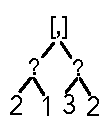
\includegraphics[scale=.25]{figures/tree1.pdf}

\noindent
At each choice point we can go either left or right, making such a decision
at each points leads to visit one particular tuple.

\hspace{-2mm}{\small
\begin{tabular}{@{}l@{~}ll@{~}ll@{~}ll@{~}l}
\begin{minipage}{1.2cm}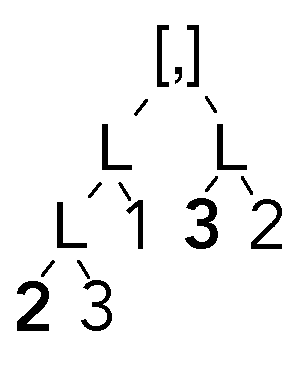
\includegraphics[scale=.25]{figures/tree2.pdf} 
\end{minipage} &  $ =   \tuple{p_2,p_3} $ &
\begin{minipage}{1.2cm}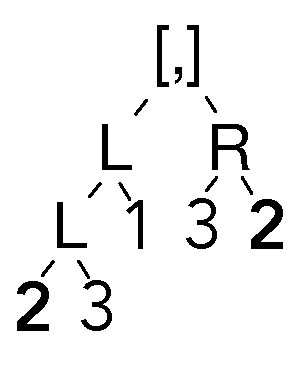
\includegraphics[scale=.25]{figures/tree3.pdf} 
\end{minipage} &  $ =   \tuple{p_2,p_2} $ 
&\begin{minipage}{1.2cm}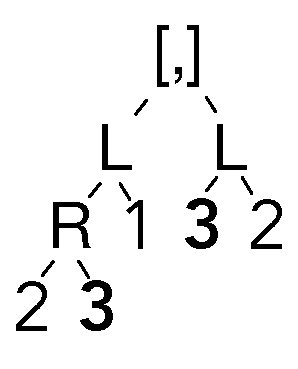
\includegraphics[scale=.25]{figures/tree4.pdf} 
\end{minipage} &  $ =   \tuple{p_2,p_3} $ \\
\begin{minipage}{1.2cm}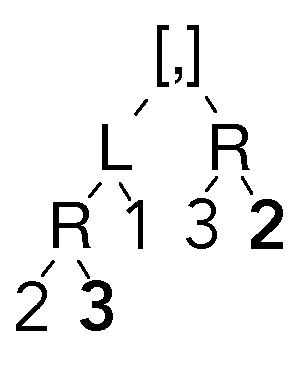
\includegraphics[scale=.25]{figures/tree5.pdf} 
\end{minipage} &  $ =   \tuple{p_2,p_2} $  &
\begin{minipage}{1.2cm}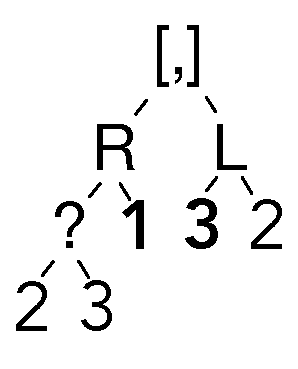
\includegraphics[scale=.25]{figures/tree6.pdf} 
\end{minipage} &  $ =   \tuple{p_3,p_2} $ 
&\begin{minipage}{1.2cm}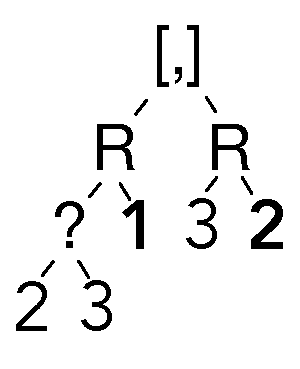
\includegraphics[scale=.25]{figures/tree7.pdf} 
\end{minipage} &  $ =   \tuple{p_3,p_3} $ 
\end{tabular}}


\noindent 
Each tuple is uniquely determined by the original type term $t$ and a choice
string $c$. In the above example, the result of iteration through the
normalized, union-free, type terms is defined by the strings \L\L\L, \L\L\R,
\L\R\L, \L\R\R, \R\L, \R\R. The length of each string is bounded by the
number of unions in a term.


The iteration sequence in the above example is thus \L\L\uL $\rightarrow$
\L\uL\R $\rightarrow$ \L\R\uL $\rightarrow$ \uL\R\R $\rightarrow$ \R\uL
$\rightarrow$ \R\R. Stepping from a choice string $c$ to the next string
consists of splitting $c$ in three, $c' \,\L\,c''$, where $c'$ can be empty
and $c''$ is a possibly empty sequence of \R.  The next string is $c'\, \R
\, c_{pad}$, that is to say it retains the prefix $c'$, toggles \L to \R,
and is padded by a sequence of \Ls.  If there is no \L in $c$, iterations has
terminated.

One step of iteration is performed by calling the \c{next} function with a
type term and a choice string. \c{next} either returns the next string in
the sequence or \c{None}. Internally, it calls on \c{step} to toggle the
last \L and shorten the string (constructing $c'\,\R$). Then it call on
\c{pad} to add the trailing sequence of \Ls (constructing $c'\,\R\,c_{pad}$).

\begin{lstlisting}
type choice = L | R

let rec next(a:typ)(l:choice list) = 
  match step l with
   | None -> None
   | Some(l') -> fst (pad a l')
\end{lstlisting}

The \c{step} function delegates to \c{toggle} the job of flipping the last
occurrence of \L. For ease of programming, it reverses the choice string so
that \c{toggle} can be written as simple recursion without an accumulator.
If the given choice string has no \L, then \c{toggle} returns empty, and
\c{step} returns \c{None}.

\begin{lstlisting}
let step (l:choice list) =
  match rev (toggle (rev l)) with
  | [] -> None
  | hd::tl -> Some(hd::tl)

let rec toggle = function
  | [] -> []    
  | L::tl -> R::tl
  | R::tl -> toggle tl
\end{lstlisting}

The \c{pad} function take a type term and a choice string to be padded. It
returns a pair, the first element is the padded string and the second is
remaining string. \c{pad} traverses the term, visiting both side of each
tuple, and for unions it uses the given choice string to direct its visit.
Each union encountered consumes a character out of the input string, once
the string is fully consumed, any remaining unions are treated as if there
was a \L. The first component of the returned value is the choice given as
argument extended with a number of \L corresponding to the number of unions
encountered after string ran out.

\begin{lstlisting}
let rec pad = function
   | (Prim i,l) -> ([],l)
   | (Tuple(t,t'),l) -> 
      let (h,tl) = pad t l in
      let (h',tl') = pad t' tl in (h @ h',tl')
   | (Union(t,_),L::r) -> 
      let (h,tl) = pad t r in (L::h,tl)
   | (Union(_,t),R::r) -> 
      let (h,tl) = pad t r in (R::h,tl)
   | (Union(t,_),[]) -> (L::(fst(pad t [])),[])
\end{lstlisting}

To obtain the initial choice string, the string only composed of \Ls, it
suffices to call \c{pad} with the type term under consideration and an empty
list. The first element of the returned tuple is the initial choice
string. For convenience, we define the function \c{initial} for this.

\begin{lstlisting}
let initial(t:typ) = fst (pad t [])
\end{lstlisting}

%%%%%%%%%%%%%%%%%%%%%%%%%%%%%%%%%%%%%%
\subsection{Subtyping with Iteration}

Subtyping visits union-free type terms using choice strings to iterate.  The
\c{subtype} function takes two type terms, \c a and \c b, and returns true
if they they are related by subtyping. It does this by iterating over all
union-free type terms in \c a, and checking that for each of them, there
exists a union-free type term in \c b that is a super-type.

\begin{lstlisting}
let subtype(a:typ)(b:typ) = allexists a b (initial a)
\end{lstlisting}

The \c{allexists} function take two type terms, \c a and \c b, and a choice
string \c f, and return true if \c a is a subtype of \c b for the iteration
sequence starting at \c f. This is achieved by recursively testing that for
each union-free type term in \c a (induced by \c a and the current value of
\c f), there exists a union-free super-type in \c b.

\begin{lstlisting}
let rec allexists(a:typ)(b:typ)(f:choice list) =
  match exists a b f (initial b) with 
  | true -> (match next a f with
             | Some ns -> allexists a b ns 
             | None -> true) 
  | false -> false
\end{lstlisting}

Similarly, the \c{exists} function takes two type terms, \c a and \c b, and
two choice strings, \c f and \c e. It returns true if there exists in \c b, a
union-free super-type of the type specified by \c f in \c a. This is done by
recursively iterating through \c e. The determination if two terms are
related is delegated to the \c{sub} function.

\begin{lstlisting}
type res = NotSub | IsSub of choice list * choice list

let rec exists(a:typ)(b:typ)(f:choice list)(e:choice list) =
 match sub a b f e with 
  | IsSub(_,_) -> true 
  | NotSub -> 
     (match next b e with
      | Some ns -> exists a b f ns 
      | None -> false) 
\end{lstlisting}

Finally, the \c{sub} function take two type terms and two choice strings and
return a value of type \c{res} which can be \c{NotSub} to indicate that the
types are not subtypes or \c{IsSub(_,_)} when they are.  If the two types
are primitives, then they are only subtypes if they are equal.  If the types
are tuples, they are subtypes is both of their elements are subtypes. Note
that the return type of \c{sub}, when successful, hold the unused choice
strings for both type arguments. When confronted with a union, \c{sub} will
follow the choice strings to decide which branch to take. Consider for
instance the case when the first type term is \c{Union(t1,t2)} and the
second is type \c{t}, if the first element of the choice string is an \L,
then \c{t1} and \c{t} will be checked, otherwise \c{sub} will check \c{t2}
and \c{t}.

\begin{lstlisting}
let rec sub = function
 | (Prim i,Prim j,f,e) -> if i==j then IsSub(f,e) else NotSub
 | (Tuple(a1,a2), Tuple(b1,b2),f,e) ->
    (match sub a1 b1 f e with
     | IsSub(f', e') -> sub a2 b2 f' e'
     | NotSub -> NotSub)
 | (Union(a,_),b,L::f,e) -> sub a b f e
 | (Union(_,a),b,R::f,e) -> sub a b f e
 | (a,Union(b,_),f,L::e) -> sub a b f e
 | (a,Union(_,b),f,R::e) -> sub a b f e
\end{lstlisting}

%%%%%%%%%%%%%%%%%%%%%%%%%%%%%%%%%%%%%%
\subsection{Further optimization}

We have presented an implementation that used lists to represent choice
strings. It thus required allocation when adding elements to the list and
for reversing the list. In Julia, choice strings are represented by bit
vectors of size bounded by the number of unions in each type term.  Once
that size is known and the bit vector is created, no further allocation is
required.

%%%%%%%%%%%%%%%%%%%%%%%%%%%%%%%%%%%%%%
%%%%%%%%%%%%%%%%%%%%%%%%%%%%%%%%%%%%%%
%%%%%%%%%%%%%%%%%%%%%%%%%%%%%%%%%%%%%%
\section{Correctness and Completeness of Subtyping}

To prove the correctness of Julia's subtyping we take the following general
approach. We start by giving a denotational semantics for types from which
we derive a definition of semantic subtyping. Then we easily prove that a
normalization-based subtyping algorithm is correct and complete. Rather than
directly working with the notion of choice strings as iterators over types,
we start with a simpler structure, namely that of iterators over the trees
induced by type terms. We prove correct and complete a subtype algorithm
that uses these simpler iterators. Finally, we establish a correspondance
between tree iterators and choice list iterators. This concludes our proof
of correctness and completeness, details can be found in the Coq
mechanization.

The denotational semantics we use for types is as follows:

\vspace{-5mm}
\begin{align*}
\denotes{p_i} &= \{p_i\} \\
\denotes{\union{t_1}{t_2}} &= \denotes{t_1} \cup \denotes{t_2} \\
\denotes{\tuplet{t_1}{t_2}} &= \{\tuplet{t'_1}{t'_2} \,|\, t_1' \in \denotes{t_1},  t_2' \in \denotes{t_2'}\}
\end{align*}
\vspace{-5mm}

\noindent
We define subtyping as follows, if $\denotes{t}\subseteq\denotes{t'}$, then
$t<:t'$.  This leads to the definition of subtyping in our restricted language.

\begin{definition}
The subtyping relation $t_1 <: t_2$ holds iff $\forall t_1' \in
\denotes{t_1}, \exists\, t_2' \in \denotes{t_2}, t_1' =
t_2'$.\label{dfn:scr}
\end{definition}

\noindent
Note that the use of equality for relating types is a simplification
afforded by the structure of primitive types.

%%%%%%%%%%%%%%%%%%%%%%%%%%%%%%%%%%%%%%%%%%
\subsection{Subtyping with Normalization}

The correctness and completeness of the normalization-based subtyping
algorithm of Section~\ref{normalize} requires proving that the \c{normalize}
function returns all union-free type terms.

\begin{lemma}[NF Equivalence]\label{lem:equiv_ndet}
$t' \in \denotes{t}$ iff $t' \in \c{normalize}~ t$.
\end{lemma}

\noindent
Theorem~\ref{nsf} states that the \c{subtype} relation of
Section~\ref{normalize} abides by Definition~\ref{dfn:scr} because it uses
\c{normalize} to compute the set of union-free type terms for both argument
types, and directly checks subtyping.

\begin{theorem}[NF Subtyping]\label{nsf}
For all  a and b, \c{subtype} a b iff $a <: b$.
\end{theorem}

\noindent
Therefore, normalization based subtyping is correct against our definition.


%%%%%%%%%%%%%%%%%%%%%%%%%%%%%%%%%%%%%%
\subsection{Subtyping with Tree Iterators}

Reasoning about iterators that use choice strings, as described in
Section~\ref{cs}, is tricky as it requires simultaneously reasoning about
the structure of the type term and the validity of the choice string that
represents the iterator's state. Instead, a tree iterator ties the two
together and thus makes reasoning simpler.

A tree iterator is a representation of the iteration state embedded in a
type term. Thus a tree iterator yields a union-free tuple, and given a type
term, a tree iterator can either step to a successor state or is a terminal
state. Recalling the graphical notation of Section~\ref{cs}, we can
represent the state of iteration as a combination of type term and a choice
or, equivalently as an tree iterator.

\medskip
{\small
\begin{tabular}{@{}l@{~}ll@{~}ll@{~}ll@{~}l}
\it Choice string: &&  \multicolumn{2}{l}{\it Tree iterator:}\\[2mm]
\begin{minipage}{1.2cm}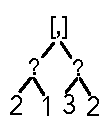
\includegraphics[scale=.25]{figures/tree1.pdf} 
\end{minipage} , \R\L & $ =   \tuple{p_1,p_3} $ 
&\begin{minipage}{1.2cm}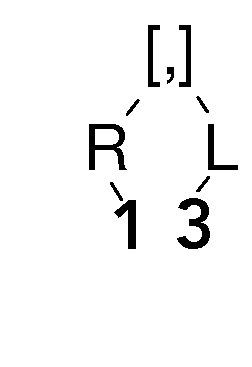
\includegraphics[scale=.25]{figures/tree8.pdf}
\end{minipage}& $=\tuple{p_1,p_3}$
\end{tabular}}

\noindent
We define tree iterators dependently on the type that they iterate over. The
possible states are \c{IPrim} at primitives, \c{ITuple} at tuples, and for
unions either \c{ILeft} or \c{IRight}.

\begin{lstlisting}
Inductive iter: Typ -> Set :=
| IPrim : forall i, iter (Prim i)
| ITuple : forall t1 t2, iter t1 -> iter t2 -> iter (Tuple t1 t2)
| ILeft : forall t1 t2, iter t1 -> iter (Union t1 t2)
| IRight : forall t1 t2, iter t2 -> iter (Union t1 t2).
\end{lstlisting}

We can then define a stepping function for tree iterators that proceeds in a
depth-first, right-to-left order.  We have four cases to worry about. For a
primitive type, there is no successor state. A tuple steps its second child;
if that has no successor step, then it steps its first child and reset the
second child. When given a \c{ILeft} or an \c{IRight} it tries step it only
child. If the child has no successor, an \c{ILeft} steps to an \c{IRight}
and its child is set to the right child of the corresponding node in the
type term.

\begin{lstlisting}
Fixpoint next(t:Typ)(i:iter t): option(iter t) := match i with
  | IPrim _ => None
  | ITuple t1 t2 i1 i2 =>
    match (next t2 i2) with
    | Some i' => Some(ITuple t1 t2 i1 i')
    | None =>
      match (next t1 i1) with
      | Some i' => Some(ITuple t1 t2 i' (start t2))
      | None => None
      end
    end
  | ILeft t1 t2 i1 =>
    match (next t1 i1) with
    | Some(i') => Some(ILeft t1 t2 i')
    | None => Some(IRight t1 t2 (start t2))
    end
  | IRight t1 t2 i2 => 
    match (next t2 i2) with
    | Some(i') => Some(IRight t1 t2 i')
    | None => None
    end
  end.
\end{lstlisting}

We can now define an induction principle over \c{next}. It is guaranteed to
eventually reach a state from which it cannot step.

\begin{theorem}[Tree Iterator Induction]
Let $P$ be any property of tree iterators for some type $t$.  Suppose $P$
holds of the final state, and whenever $P$ holds of a succesor state $it$
then it holds of its precursor $it'$ where $\c{next}~t~it' = it$.  Then $P$
holds of every iterator state over $t$.
\end{theorem} 


Using \verb|iter_rect|, we can implement and prove correct equivalent functions
to \verb|exists|, and \verb|allexists|. Therefore, we can prove a version of \verb|subtype|
based on iteration over choice trees.

\begin{small}\begin{verbatim}
let rec exists (a b:typ) (ib:iter b) =
    (sub a (current_type b ib)) || 
        (match next b ib with Some(ns) => exists a b ns | None => false)
let rec allexists (a b:typ) (ia:iter a) =
    (exists (current_type a ia) b (init b)) && 
        (match next a ia with Some(ns) => allexists a b ns | None => true)
let subtype (a b:typ) = allexists a b (init a)
\end{verbatim}\end{small}

\verb|exists_iter| is equivalent to the choice string based \verb|exists|,
and determines if there exists some denotationally-contained type in \verb|b|
that is a supertype of the given \verb|a|. Internally, it is implemented by 
using \verb|iter_rect| to perform induction over the list of remaining states in
the iterator for \verb|b|. If no states remain, then trivially the failing case holds.
Otherwise, it will determine if the current iterator state is a supertype of the given
\verb|a|. If it is, then it can terminate early with a successful (left) outcome. Otherwise,
it continues with the IH.

\begin{small}\begin{verbatim}
Definition forall_iter (a b : Typ) :
  { forall t, In t (clauses a) -> exists t', InType t' b /\ (BaseSubtype t t')} +
  { exists t, In t (clauses a) /\ forall t', InType t' b -> ~ (BaseSubtype t t')}.
\end{verbatim}\end{small}

\verb|forall_iter| is to \verb|allexists| what \verb|exists_iter| is to
\verb|exists|. Like \verb|exists_iter| it implements the same decision procedure
as \verb|allexists| (and internally relies upon \verb|exists_iter|), though through
the abstraction of \verb|iter_rect|.

Finally, we can define a decidable function (called \verb|subtype| in the proof)
that decides whether two types are subtypes or not. \verb|subtype| simply invokes
\verb|forall_iter| to decide subtyping.

\begin{small}\begin{verbatim}
Definition subtype(a b:Typ) : {NormalSubtype a b} + {~NormalSubtype a b}.
\end{verbatim}\end{small}

\noindent The definition of \verb|subtype| works by calling \verb|forall_iter|, then
conditioning its output to produce a result in terms of \verb|NormalSubtype|. 

We can thus decide subtyping using choices at tree nodes as our iterator state.
However, this does not yet prove correct the previous algorithm over choice strings.

%%%%%%%%%%%%%%%%%%%%%%%%%%%%%%%%%%%%%%
\subsection{Subtyping with Choice Strings}

We prove the subtyping algorithm using choice strings correct by 
showing that choice string iterators simulate tree iterators. To 
relate tree iterators to choice string iterators, we use the \c{itp} 
function, which traverses a tree iterator state and produces a choice
string using a depth-first search.

\begin{small}\begin{verbatim}
Fixpoint itp(t:Typ)(it:iter t):choice list :=
   match it with
   | IPrim _ => nil
   | ITuple t1 t2 it1 it2 => (itp t1 it1) ++ (itp t2 it2)
   | ILeft t1 _ it1 => Left :: (itp t1 it1)
   | IRight _ t2 it1 => Right :: (itp t2 it1)
   end.
\end{verbatim}\end{small}

Then, the translated input and output of the tree iterator \c{next}
function is of the form described in section~\ref{cs}. A choice tree \c{it}
that can be stepped will be turned by \c{itp} into a list of the form
\c{hd ++ (L :: tl)}, where \c{hd} is some prefix and \c{tl} is a list of 
all \Rs. If we then step \c{it} to \c{it2} using \c{next} for trees,
\c{itp} will turn \c{it2} into a list of the form \c{hd ++ (R :: tl')},
where \c{tl'} is a list consisting of all-\Ls.

\begin{lemma}[Structure of linearized {\tt next\_tree}]
\label{lem:snt}
If a explicit assignment iterator \verb|it| can take a step to \verb|it'|, then
the linearized \verb|it| consists of some prefix and a \L-choice followed by a suffix of \Rs.
The resulting \verb|it'| will then have the same prefix, a \R-choice, and a suffix of \Ls.
\end{lemma}

We can then prove that stepping a type iterator state is equivalent to
stepping the linearized versions of the state using the choice string
\c{next} function.


\begin{lemma}[Correctness of step\_ctx]
\begin{small}\begin{verbatim}
forall t it,
    step_ctx t (itp t it) = (option_map (itp t) (next_tree t it)).
\end{verbatim}\end{small}
For every type \verb|t| and type iterator \verb|it|,
stepping the choice-list equivalent of \verb|it| will
produce the same result as converting the result of stepping
\verb|it|.
\end{lemma}
\begin{proof}
If no next state exists from \verb|it|, then
\verb|itp t it| must consist solely of \Rs. Therefore, \verb|step_ctx| will be \verb|None| as 
will \verb|next_tree t it| and the theorem holds. 

Otherwise, if there is some step tha can be taken from \verb|it|, then 
the remainder follows from lemma~\ref{lem:snt}. We know that \verb|itp t it| can
be broken down into a string of the form $c\,\L\,c'$ where $c'$ is solely \Rs, and thus
the left hand side will be \verb|Some(|$c\,\R\,c''$\verb|)| where $c''$ is some amount of 
padding \Ls. By lemma~\ref{lem:snt}, the right hand side can be decomposed identically, and the theorem holds.
\end{proof}

Now, with the relevant properties proven, we can implement and prove correct
\verb|exists| and \verb|allexists| in Coq. The function names are the
same, as are the implementations up to the addition of a fuel parameter (which
is shown to be unnecessary). 

\begin{lemma}[Correctness of existential subtype checking with choice strings]
\label{lem:correxcst}
\begin{small}\begin{verbatim}
forall a b it, 
  (exists pf, exists_iter_inner a b it = inleft pf) <->
   exists n, exists a b (iterator_to_path b it) n = Some true.
\end{verbatim}\end{small}
For every two types \verb|a| and \verb|b|, the iterator-based algorithm
\verb|exists_iter_inner| will produce a proof that \verb|a| is a subtype
of \verb|b| if and only if there is an integer \verb|n| such that
 \verb|exists| given \verb|n| fuel runs producing true.
\end{lemma}
\begin{proof}

The proof proceeds by induction on the tree iterator \verb|it|. If
\verb|it| has no more steps, then \verb|exists_iter_inner| will be true
(\verb|inleft|, in this encoding) iff the current \verb|it| induces a
supertype of \verb|a|. Moreover, if \verb|it| cannot step, then neither can
\verb|itp t it|, so \verb|exits| is only true if the \verb|b| with \verb|itp t it|
is a supertype of \verb|a|. 

Otherwise, if \verb|it| can take a step, then either we find that \verb|b|
with \verb|it| and \verb|itp t it| is a supertype of \verb|a|, or we defer to
the IH.
\end{proof}

\begin{lemma}[Correctness of forall-exists subtype checking with choice strings]
\begin{small}\begin{verbatim}
forall a b it,
   (exists pf, forall_iter_inner a b it = left pf) <->
    exists n, allexists a b (itp a it) n = Some true.
\end{verbatim}
\end{small}  
For every two types \verb|a| and \verb|b|, the iterator-based algorithm
\verb|forall_iter_inner| will produce a proof that \verb|a| is a subtype
of \verb|b| if and only if there is an integer \verb|n| such that
 \verb|allexists| given \verb|n| fuel runs producing true.
\end{lemma}
\begin{proof}
The proof runs identically to that of \verb|ex_sub_corr_eq|; we run through
\verb|it| with \verb|iter_rect| stepping \verb|it| and \verb|itp t it| in sync
until the base case is reached. At each step, the functions both check that there
exists some satisfying explicit assignment or choice list for \verb|b| that is a 
supertype of \verb|a| with \verb|it| or \verb|itp t it|. 
\end{proof}

In conjunction with the negations of above theorems, the choice stack-based algorithm is provably equivalent to the
iterator-based algorithm. Using the the convenience function \verb|allexists_ex| to generate the needed fuel argument \verb|n|,
can therefore write a proof-generating subtype implementation that uses choice strings:

\begin{verbatim}
Definition stack_subtype (a b: type) : {NormalSubtype a b} + {~NormalSubtype a b}.
Proof.
  intros. destruct (allexists_ex a b).
  - left. [...]
  - right. [...]
End.
\end{verbatim}

In this manner, we can provably correctly decide subtyping with distributive unions and tuples using
the choice list based implementation of iterators.

\section{Complexity}

Worst case time complexity of Julia's subtyping algorithm and
normalization-based approaches is determined by the number of terms that
would exist in the normalized type. In the worst case, there are $2^n$
union-free tuples in the fully normalized version of a type that has $n$
unions.  Each of these tuples must always be explored. As a result, both
algorithms have worst-case $O(2^n)$ time complexity. The approaches differ,
however, in space complexity. The normalization approach computes and stores
each of the exponentially many alternatives, so also has $O(2^n)$ space
complexity. However, Julia need only store the choice made at each union,
thereby offering $O(n)$ space complexity.

Julia's algorithm improves best-case time performance.  Normalization always
experiences worst case time and space behavior as it has to precompute the
entire normalized type. Julia's iteration-based algorithm can discover the
relation between types early. In practice many queries are of the form $uft
<: union(t_1...t_n)$ where $uft$ is already union-free tuple and thus all
that Julia needs to do if find one matching tuple in $t_1 ... t_n$.

\section{Conclusion}

We have presented an algorithm for deciding subtyping relationships between
types that consist of atomic types, tuples, and unions. This algorithm is able
to decide subtyping relationships in the presence of distributive semantics
for union types without needing normalization (and therefore using linear
space) and without additionally constraining type system features.

\subsubsection*{Acknowledgments}
The authors thank Jiahao Chen for starting us down the path of understanding
Julia, and Jeff Bezanson for coming up with Julia's subtyping algorithm.  This
work received funding from the European Research Council under the European
Union's Horizon 2020 research and innovation programme (grant agreement
695412), the NSF (award 1544542 and award 1518844) and the Czech Ministry of
Education, Youth and Sports (grant agreement
CZ.02.1.01/0.0/0.0/15\_003/0000421).
 

%\bibliographystyle{plain}
\bibliography{refs}
\end{document}
